\chapter{Reflection properties of metals}

Most of the experiments probing the Casimir effect use metallic mirrors. In the
last decades the accuracy of such experiments was drastically improved and for
an accurate description it is thus essential to use a realistic description of
the reflection properties of the metals. The reflection properties of metals
are described in terms of the dielectric function $\epsilon(\omega)$. In this
chapter, we introduce the Drude model that takes finite conductivity and plasma
oscillations into account. We derive from the Drude model the plasma model
which neglects effects due to dissipation, and the model for perfect reflectors
that assumes perfect conductivity at arbitrary frequencies. Given the
dielectric function $\epsilon(\omega)$, we present the solutions of the
scattering of plane waves at a plane and a sphere.

\section{Drude model}

The Drude model is based on the assumption that the valence electrons are
detached from the atoms and can move freely within the metal. Although we
consider a quantum mechanical problem, we assume the electrons to be classical
particles. We consider an electric field with harmonic time dependence
\begin{equation}
\label{eq:drude_E}
\vec E(t) = \vec{E}(\omega) \, \e^{-\imag\omega t}.
\end{equation}
The electric field \eqref{eq:drude_E} will accelerate the electrons. If we
assume that there is some kind of linear dissipation, the velocity of an
electron is described by
\begin{equation}
\me\dot{\vec{v}} + \gamma \me \vec{v} = -\qe \vec E,
\end{equation}
where $\me$ is the (effective) mass of an electron and $\gamma$ is called
relaxation frequency. The steady-state solution is given by
\begin{equation}
\vec v = \frac{-\qe}{\me(\gamma-\imag\omega)}.
\end{equation}
In an isotropic and linear medium electric field and current density are parallel
with the factor of proportionality given by the AC conductivity $\sigma(\omega)$.
For the Drude model we find
\begin{equation}
\vec j \equiv \sigma(\omega) \vec E(\omega) = -\nee\qe \vec v = \frac{\nee \qe^2}{\me(\gamma-\imag\omega)} \vec E,
\end{equation}
where the AC conductivity is given by
\begin{equation}
\sigma(\omega) \equiv \frac{\nee\qe^2}{\me(\gamma-\imag\omega)} = \frac{\sigma_0}{1-\frac{\imag\omega}{\gamma}}, \\
\sigma_0 \equiv \sigma(\omega=0) = \frac{\nee\qe^2}{\me\gamma}.
\end{equation}
Maxwell's equations inside the metal are
\begin{equation}
\vec \nabla \cdot \vec E = 0, \\
\vec \nabla \cdot \vec B = 0, \\
\vec \nabla \times \vec E = -\frac{\partial\vec B}{\partial t}, \\
\vec \nabla \times \vec B = \mu_0 \vec j + \epsilon_0 \mu_0 \frac{\partial \vec E}{\partial t}.
\end{equation}
The electric field obeys the wave equation
\begin{equation}
\label{optical_drude_wave}
\vec\nabla \times \left(\nabla\times \vec E\right) = -\vec\nabla^2 \vec E = 
- \frac{\partial}{\partial t} \left(\mu_0 \vec j + \frac{1}{\c^2}\frac{\partial}{\partial t} \vec E\right) \equiv
\frac{\omega^2}{\c^2} \epsilon(\omega) \vec E,
\end{equation}
where the complex dielectric function $\epsilon(\omega)$ is given by
\begin{equation}
\label{eq:drude_drude_complex}
\epsilon(\omega) \equiv 1-\frac{\omega_P^2}{\omega(\omega+\imag\gamma)}, \\
\omega_P^2 \equiv \frac{\nee\qe^2}{\epsilon_0 \me}.
\end{equation}
For $\omega\gg\omega_P\gg\gamma$ the metal becomes transparent. A more detailed
discussion of the properties of metals and the Drude model can be found in
standard textbooks of solid state physics like \cite{ashcroft1976solid}.

In section \ref{section_wick} we will perform a Wick rotation. The dielectric
function is then evaluated at imaginary frequencies $\omega=\imag\xi$. We are
thus lead to study the dielectric function at imaginary frequencies. At
imaginary frequencies the dielectric function becomes a real-valued function
\begin{equation}
\epsilon(\imag\xi) = 1+\frac{\omega_P^2}{\xi(\xi+\gamma)}.
\end{equation}
The high and low frequency limits are given by
\begin{align}
\label{eq:drude_approx_drude_xih}
\epsilon(\imag\xi) &\simeq 1+\frac{\omega_P^2}{\xi^2}   & &\text{for} \sep \xi\gg\gamma, \\
\label{eq:drude_approx_drude_xi0}
\epsilon(\imag\xi) &\simeq \frac{\omega_P^2}{\gamma\xi} & &\text{for} \sep \xi\ll\gamma.
\end{align}


\section{Plasma model and perfect reflectors}

\begin{figure}
\begin{center}
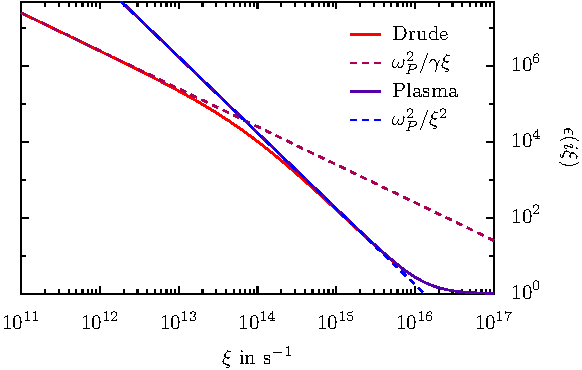
\includegraphics[scale=1]{plots/drude_log.pdf}
\end{center}

\caption{Drude and plasma model with parameters
$\omega_\text{P}=1.32\cdot10^{16} \, \mathrm{s}^{-1}$, $\gamma=6.90\cdot10^{13}
\, \mathrm{s}^{-1}$, corresponding to silver \cite{PhysRevB.65.165432}. The
upper solid line corresponds to the plasma model, the lower solid line to the
Drude model. The dashed lines correspond to the low frequency approximations of
the Drude and plasma model. The dielectric functions for Drude and the plasma
model are plotted together with the approximations
\eqref{eq:drude_approx_drude_xi0} and \eqref{eq:drude_approx_plasma} for
imaginary frequencies.}
\label{fig:optical_properties_drudeplasma}
\end{figure}

The plasma model neglects effects due to dissipation and can be obtained from
the Drude model by taking the limit $\gamma\to0$. The dielectric function at
imaginary frequencies becomes
\begin{equation}
\epsilon(\imag\xi) = 1 + \frac{\omega_P^2}{\xi^2}
\end{equation}
and corresponds to the high frequency limit of the Drude model. In other words,
Drude and plasma model agree for frequencies $\xi\gg\gamma$.
The low frequency limit $\xi\ll\omega_P$ is given by
\begin{equation}
\label{eq:drude_approx_plasma}
\epsilon(\imag\xi) \simeq \frac{\omega_P^2}{\xi^2}.
\end{equation}
In Fig. \ref{fig:optical_properties_drudeplasma} we show the dielectric
functions of the Drude and plasma models for silver and its approximations for
imaginary frequencies.

The model of perfect reflectors can be obtained from the plasma model by taking the limit
$\omega_P\to\infty$. The dielectric function $\epsilon(\imag\xi)=\infty$ is infinite at
arbitrary frequencies.

\section{Fresnel coefficients}
\label{section_optical_properties_fresnel}

The reflection and transmission coefficients for an incident plane wave at a
flat, planar and homogenous interface between dielectrics are called Fresnel
coefficients. We will consider a vacuum--metal interface at $z=0$. The Fresnel
coefficients are obtained by solving the boundary value problem at the
interface. TE- and TM-polarization are well adapted to this boundary value
problem and the reflection of a plane wave yields
\begin{equation}
\ket{ \vec k, \omega, -\phi, p}_\text{ref} = r_p(\omega,\vec k) \ket{ \vec k, \omega, \phi, p}_\text{in}.
\end{equation}
The subscript ``in'' denotes the incident wave, the subscript ``ref'' the
reflected wave. The frequency $\omega$, the wave vector in the $xy$-plane
$\vec k$, and the polarization $p={\TE,\TM}$ remain constant during the
scattering, but the direction of propagation changes. The reflection
coefficient is given by the Fresnel coefficient $r_p$.

The Fresnel coefficients at imaginary frequencies $\omega=\imag\xi$ are \cite{jackson}
\begin{equation}
\label{eq:drude_fresnel_rtetm}
r_\text{TE}(\imag\xi, k) = \frac{1-\beta}{1+\beta} \\
r_\text{TM}(\imag\xi, k) = \frac{\epsilon(\imag\xi) - \beta}{\epsilon(\imag\xi) + \beta},
\end{equation}
where
\begin{equation}
\label{eq:drude_fresnel_beta}
\beta = \sqrt{1+\frac{\epsilon(\imag\xi)-1}{\cos^2{\theta^\pm}}}.
\end{equation}
Because of the dispersion relation
\begin{equation}
k_z^2 = \frac{\omega^2}{\c^2} - k^2 = -\frac{\xi^2}{\c^2} - k^2,
\end{equation}
the $z$-component of the wave vector $k_z$ also becomes imaginary for imaginary
frequencies. For this reason, we define
\begin{equation}
k_z \equiv \imag \kappa, \\
\kappa \equiv \sqrt{\frac{\xi^2}{\c^2}+k^2},
\end{equation}
where $\kappa \in \mathbb{R}$. The relations \eqref{eq:notation_cossintheta}
become
\begin{equation}
\sin\theta^\pm = -\imag \frac{\c k}{\xi}, \\
\cos\theta^\pm = \pm \frac{\c \kappa}{\xi},
\end{equation}
and we can express $\beta$ in terms of $\xi$, $\kappa$ and $\epsilon(\imag\xi)$:
\begin{equation}
\beta = \sqrt{1+\frac{\xi^2}{\c^2\kappa^2}\left[\epsilon(\imag\xi)-1\right]}
\end{equation}

The Fresnel coefficients for perfect reflectors are obtained by taking the
limit $\epsilon\to\infty$. The coefficients become
\begin{equation}
r^\text{perf}_\TM = -r^\text{perf}_\TE = 1.
\end{equation}
and are independent of $\xi$ and $\kappa$.

The properties of the Fresnel coefficients for low frequencies deserve a
careful analysis for Drude and plasma reflectors. For $\xi\to0$ the parameter
$\beta$ becomes in the Drude model
\begin{equation}
\beta^\text{Drude} = \sqrt{1 + \frac{\xi \omega_P^2}{\c^2 \kappa (\xi+\gamma)}} \overset{\xi\to0}{=} 1.
\end{equation}
The dielectric function diverges for $\xi\to0$ and the Fresnel coefficients
become
\begin{equation}
\lim_{\xi\to0} r_\TE^\text{Drude} = 0, \\
\lim_{\xi\to0} r_\TM^\text{Drude} = 1.
\end{equation}
For Drude metals we see that the Fresnel coefficients become universal and
independent of the particular properties of the metal for $\xi\to0$. This is
not true for the plasma model. In the plasma model $\beta$ becomes
\begin{equation}
\beta^\text{plasma} = \sqrt{1+\frac{\omega_P^2}{\c^2\kappa^2}} \overset{\xi\to0}{=} \sqrt{1+\frac{\omega_P^2}{\c^2\kappa^2}}
\end{equation}
and the Fresnel coefficients are given by
\begin{equation}
\label{eq:drude_rteplasmaxi0}
\lim_{\xi\to0} r_\TE^\text{plasma} = \frac{1-\sqrt{1+\frac{\omega_P^2}{\c^2\kappa^2}}}{1+\sqrt{1+\frac{\omega_P^2}{\c^2\kappa^2}}}, \\
\lim_{\xi\to0} r_\TM^\text{plasma} = 1.
\end{equation}
In contrast to the Drude model, the Fresnel coefficient for the TE mode is not universal and
still depends on $\kappa$ and $\omega_P$ in the plasma model. For this reason, the limits
$\xi\to0$ and $\gamma\to0$ do not interchange:
\begin{align}
\lim_{\xi\to 0} \lim_{\gamma\to0} r_\TE^\text{Drude} &= \lim_{\xi\to 0} r_\TE^\text{plasma} = \frac{1-\sqrt{1+\frac{\omega_P^2}{\c^2\kappa^2}}}{1+\sqrt{1+\frac{\omega_P^2}{\c^2\kappa^2}}} \\
\lim_{\gamma\to0} \lim_{\xi\to 0} r_\TE^\text{Drude} &= 0
\end{align}
However, the limits $\xi\to0$ and $\omega_P\to\infty$ do interchange:
\begin{align}
\lim_{\xi\to 0} \lim_{\omega_P\to\infty} r_\TE^\text{plasma} &= \lim_{\xi\to 0} r_\TE^\text{perf} = -1 \\
\lim_{\omega_P\to\infty} \lim_{\xi\to 0} r_\TE^\text{plasma} &= \lim_{\omega_P\to\infty} \frac{1-\sqrt{1+\frac{\omega_P^2}{\c^2\kappa^2}}}{1+\sqrt{1+\frac{\omega_P^2}{\c^2\kappa^2}}} = -1
\end{align}
This means that there is no continous transition for the TE-Fresnel coefficient
from the Drude to the plasma model. As a consequence, there is neither a
continous transition from the Drude to the plasma model, nor a continous
transition from the Drude model to the model of perfect reflectors.


\section{Mie coefficients}

Mie scattering describes the scattering of electromagnetic waves by a sphere.
The Mie coefficients for complex frequencies $\omega=\imag\xi$ are given by
\cite{bohrenhuffman, Durand, PhysRevA.83.039905}
\begin{equation}
a_\ell(\imag\chi) = (-1)^{\ell+1} \frac{\pi}{2} \, \frac{n^2 s_\ell^{(a)}-s_\ell^{(b)}}{n^2 s_\ell^{(c)}-s_\ell^{(d)}}, \\
b_\ell(\imag\chi) = (-1)^{\ell+1} \frac{\pi}{2} \, \frac{s_\ell^{(a)}-s_\ell^{(b)}}{s_\ell^{(c)}-s_\ell^{(d)}},
\end{equation}
using the abbrevations
\begin{align}
\nonumber
s_\ell^{(a)} &= I_{\ell+1/2} (n\chi) \left[ \ell I_{\ell+1/2}( \chi)- \chi I_{\ell-1/2}( \chi) \right],
&s_\ell^{(b)} &= I_{\ell+1/2}( \chi) \left[ \ell I_{\ell+1/2}(n\chi)-n\chi I_{\ell-1/2}(n\chi) \right], \\
s_\ell^{(c)} &= I_{\ell+1/2} (n\chi) \left[ \ell K_{\ell+1/2}( \chi)+ \chi K_{\ell-1/2}( \chi) \right],
&s_\ell^{(d)} &= K_{\ell+1/2}( \chi) \left[ \ell I_{\ell+1/2}(n\chi)-n\chi I_{\ell-1/2}(n\chi) \right],
\end{align}
where $n=\sqrt{\epsilon}$ is the refraction index of the sphere, and $\chi =
\xi R/\c$. Properties of the modified Bessel functions $I_\nu(x)$ and
$K_\nu(x)$ are briefly described in appendix
\ref{appendix_modified_bessel_functions}. We also want to point out that the
Mie coefficients are independent of $\vec k$ and $m$, which is a consequence of
the rotational symmetry.

\begin{figure}
\begin{center}
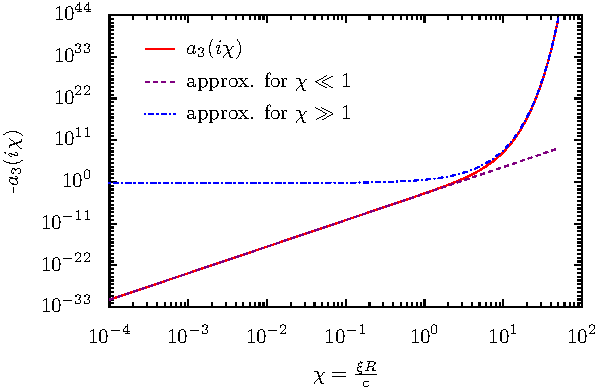
\includegraphics[scale=1]{plots/mie.pdf}
\end{center}
\caption{Mie coefficient $a_3(\imag\chi)$ with approximations for a perfect
reflector. For small arguments the behaviour is polynomial, for large arguments
it is exponential. The Mie coefficient covers about 80 orders of magnitude in
the range $10^{-4}\lesssim\chi\lesssim 10^2$.}
\label{fig:optical_properties_mie}
\end{figure}

We obtain the Mie coefficients for perfect reflectors by taking the limit
$\epsilon~\to~\infty$ and find
\begin{align}
a_\ell^\text{perf}(\imag\chi) &= \frac{\pi}{2} (-1)^{\ell+1} \frac{ \ell\,I_{\ell+1/2}(\chi) - \chi\,I_{\ell-1/2}(\chi) }{ \ell\,K_{\ell+1/2}(\chi) + \chi\,K_{\ell-1/2}(\chi) }, \\
b_\ell^\text{perf}(\imag\chi) &= \frac{\pi}{2} (-1)^{\ell+1} \frac{ I_{\ell+1/2}(\chi)}{ K_{\ell+1/2}(\chi) }.
\end{align}
For $\xi R/\c \ll 1$ the Mie coefficients $a_\ell$,$b_\ell$ can be simplified
using the approximations of the Bessel functions \eqref{eq:appendix_bessel_approx_small}
\begin{equation}
\label{eq:scattering_ps_mie_approx}
a_\ell^\text{perf} \simeq a_{\ell,0}^\text{perf} \, \left(\frac{\chi}{2}\right)^{2\ell+1}, \\
b_\ell^\text{perf} \simeq b_{\ell,0}^\text{perf} \, \left(\frac{\chi}{2}\right)^{2\ell+1},
\end{equation}
where
\begin{equation}
\label{eq:scattering_ps_mie_prefactors}
a_{\ell,0}^\text{perf} \equiv (-1)^{\ell}   \frac{\pi\left( 1 + \frac{1}{\ell}\right)}{\Gamma\left(\ell+\frac{1}{2}\right) \Gamma\left(\ell+\frac{3}{2}\right)}, \\
b_{\ell,0}^\text{perf} \equiv (-1)^{\ell+1} \frac{\pi}{\Gamma\left(\ell+\frac{1}{2}\right)\,\Gamma\left(\ell+\frac{3}{2}\right)}.
\end{equation}
For $\xi R / \c \gg 1$ the Mie coefficients can be approximated
using \eqref{eq:appendix_bessel_approx_large}
\begin{equation}
\label{eq:optical_properties_mie_large}
a_\ell(\imag\chi) \simeq (-1)^\ell \frac{(\chi-\ell)\e^{2\chi}}{2(\chi+\ell)} \overset{\chi\gg\ell}{\simeq} (-1)^\ell \frac{\e^{2\chi}}{2}, \\
b_\ell(\imag\chi) \simeq (-1)^{\ell+1} \frac{\e^{2\chi}}{2}.
\end{equation}
We see that for low frequencies the Mie coefficients show polynomial, and for
high frequencies exponential behaviour. Fig. \ref{fig:optical_properties_mie}
depicts the Mie coefficient $a_3$ for a perfect reflector along with its high
and low frequency approximations.
